% Created 2011-08-25 Thu 13:06
\documentclass[11pt,english]{article}
\usepackage[utf8]{inputenc}
\usepackage[T1]{fontenc}
\usepackage{fixltx2e}
\usepackage{graphicx}
\usepackage{longtable}
\usepackage{float}
\usepackage{wrapfig}
\usepackage{soul}
\usepackage{textcomp}
\usepackage{marvosym}
\usepackage{wasysym}
\usepackage{latexsym}
\usepackage{amssymb}
\usepackage{hyperref}
\tolerance=1000
\usepackage{color}
\usepackage{listings}

\usepackage{lmodern}
\renewcommand{\sfdefault}{lmss}
\renewcommand{\ttdefault}{lmtt}

% needed packages
\usepackage{amsmath}
\usepackage{amssymb}
\usepackage{amsthm}
\usepackage{babel}
\usepackage{epsfig}
\usepackage[T1]{fontenc}
\usepackage{fixltx2e}
\usepackage{float}
%\usepackage{floatflt}
\usepackage{graphics}
\usepackage{graphicx}
\usepackage[utf8]{inputenc}
\usepackage{latexsym}
\usepackage{longtable}
\usepackage{makeidx}
\usepackage{marvosym}
\usepackage{multicol}
%\usepackage{pslatex}
\usepackage{rotating}
%\usepackage{showidx}
\usepackage{soul}
\usepackage{srcltx}
\usepackage{stmaryrd}
\usepackage{subfig}
\usepackage{textcomp}
%\usepackage{theorem}
%\usepackage[subfigure]{tocloft}
\usepackage{txfonts}
\usepackage{upgreek}
\usepackage{url}
\usepackage{varioref}
%\usepackage{wasysym}
\usepackage{wrapfig}


% Page setup
\usepackage[paperwidth=8.5in,paperheight=11in]{geometry}
\geometry{verbose,tmargin=0.5in,bmargin=0.5in,lmargin=1in,rmargin=1in}




% PDF settings
%\usepackage[hyperref,x11names]{xcolor}
\usepackage{hyperref}
\hypersetup{pdftitle={STAT 5840: Statistical Computing},
 		pdfauthor={G. Jay Kerns}, 
		linkcolor=Firebrick4, 
		citecolor=black, 
		urlcolor=SteelBlue4}

% Listings setup
%\usepackage{color}
%\usepackage{listings}
%\lstset{basicstyle={\ttfamily},
%	language=R,
%	breaklines=true,
%	breakatwhitespace=true,
%	keywordstyle={\ttfamily},
%	numberstyle = {\ttfamily},
%	morestring=[b]"
%}



%  user defined commands
% special operators
\renewcommand{\P}{\mathrm{I\hspace{-1.5pt}P}}
\newcommand{\E}{\mathrm{I\hspace{-1.5pt}E}}
\renewcommand{\vec}[1]{\mbox{\boldmath$#1$}}

% special symbols
\newcommand{\me}{\mathrm{e}}
\newcommand{\R}{\mathbb{R}}
\newcommand{\diff}{\mathrm{d}}
\newcommand{\ybar}{\overline{y}}
\newcommand{\xbar}{\overline{x}}
\newcommand{\Xbar}{\overline{X}}
\newcommand{\Ybar}{\overline{Y}}





\providecommand{\alert}[1]{\textbf{#1}}

\title{Accept-Reject Algorithm}
%\author{G. Jay Kerns}
\date{STAT 5840: Summer 2011}

\begin{document}

\maketitle

\thispagestyle{empty}

We cover the standard Normal density with a Cauchy proposal density and use the accept-reject algorithm.  We copy-paste the \texttt{rand\_norm} function at the command prompt in \texttt{R}.


\begin{verbatim}
rand_norm <- function(n){
  M <- 1.5203;           # bound used in A/R algorithm
  i <- 0; N <- 0;        # initialization and storage
  z <- rep(0, times = n);

  while(i < n){                      # keep going until n accepts
      x <- tan(pi*(runif(1) - 0.5))  # simulate a Cauchy
      u <- runif(1)                  # simulate a Uniform
      f <- 1/sqrt(2*pi)*exp(-x^2/2)  # compute f(x)
      g <- 1/pi/(1+x^2)              # compute g(x)
      if (u <= f/M/g){
        i <- i + 1;            # got another accept
        z[i] <- x;             # save this one
      }
    N <- N + 1                 # keep track of num trials
  }
list(z = z, accept = n/N)                     
}
\end{verbatim}



After the copy-paste we can run the function with the following.

\begin{verbatim}
tmp <- rand_norm(10000)
tmp$accept
\end{verbatim}




\begin{verbatim}
 [1] 0.652103
\end{verbatim}


The acceptance rate is around 65\%.  We see plots below.



\begin{figure}[h!]
\centering
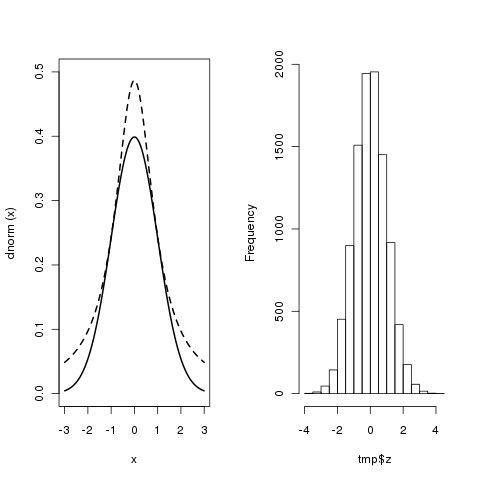
\includegraphics[width=5in, height=2in,]{ARalgo.png}
\caption{\label{fig:yplot}Plot of the target/proposal densities, plus histogram}
\end{figure}


\end{document}